%%% Simuleirng af optimering af udgangsfilter %%%

\subsection{Udgangsfilter}
Simulering af det optimerede udgangsfilter, gøres ved at modulere selvinduktionerne i ledningerne, som er en del af filteret. Kredsløbet for dette ses på figur~\ref{fig:diagram_udgangsfilter_3}. Her er filteret moduleret som de fire kondensatorer i parallel, og med selvinduktionerne på $30nH$ i ledningerne mellem dem. 

\begin{figure}[H]
	\center
	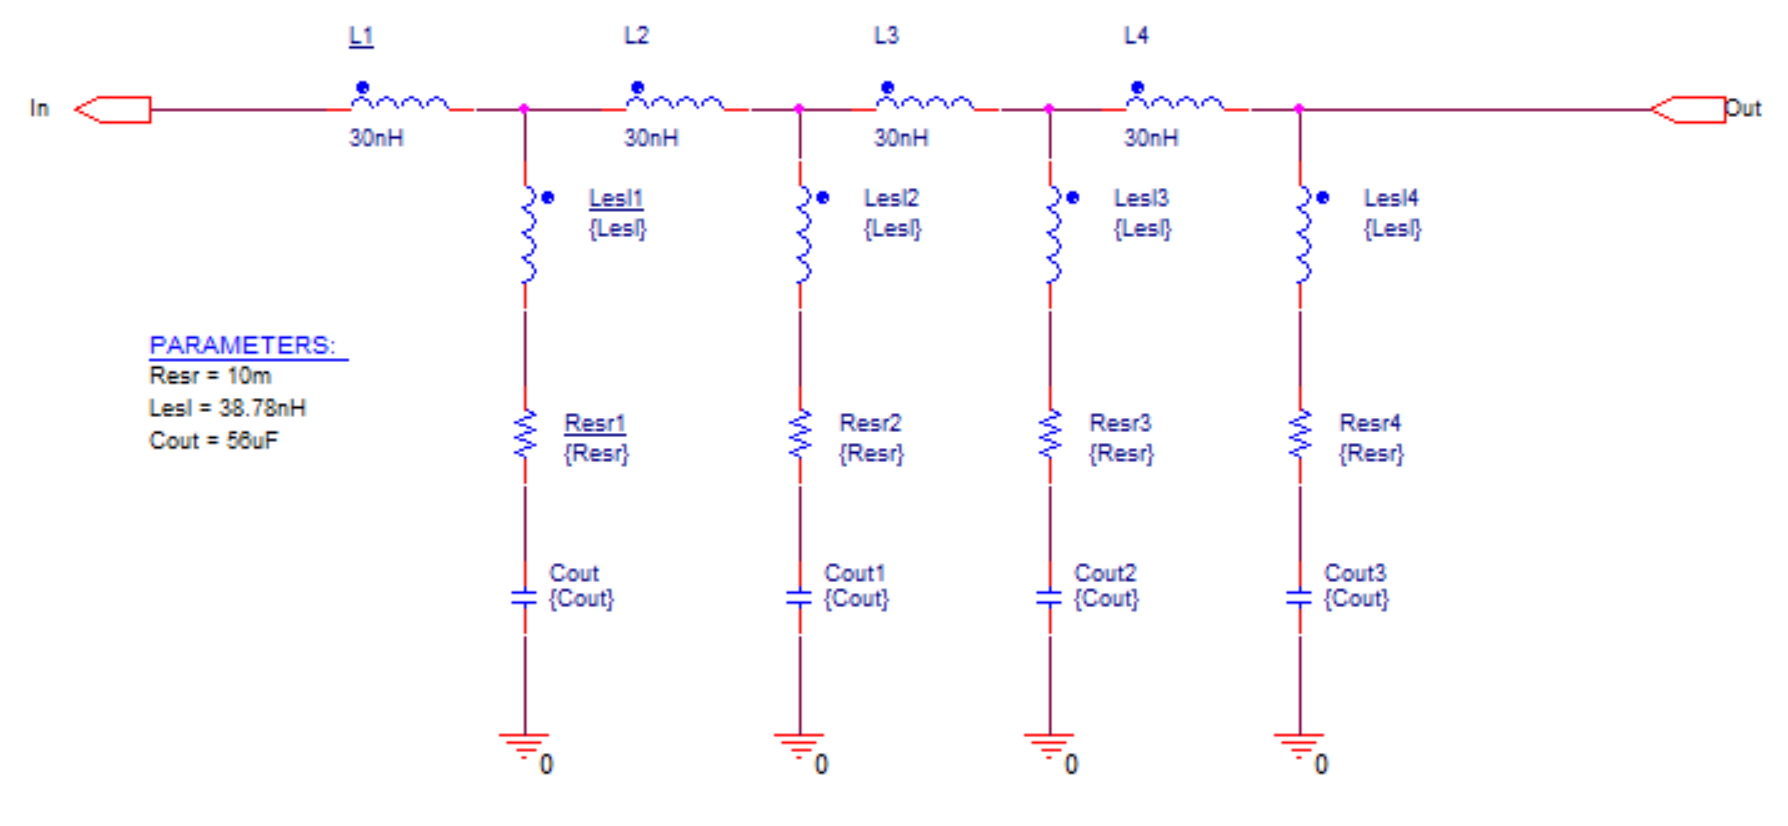
\includegraphics[max width=0.9\linewidth]{/tex/3iteration/billeder/Simulering/diagram_udgangsfilter.png}
	\caption{Diagram for udgangsfilter}
	\label{fig:diagram_udgangsfilter_3}
\end{figure}

\noindent Simuleringen er foretaget på figur~\ref{fig:simulering_udgangsfilter_U} og \ref{fig:simulering_udgangsfilter_M}. Her vises udgangssignalet før filteret på figur~\ref{fig:simulering_udgangsfilter_U}. Her aflæses der en spike på ca. $10V pk-pk$. Det er en større spike end ved realiseringen i 2. iteration, men viser at det er noget der skal filtreres væk. Figur~\ref{fig:simulering_udgangsfilter_M} viser signalet efter filteret. Her aflæses spiken til ca. $900mV pk-pk$. Det viser, at den teoretiske funktionalitet er opnået ved, at flytte udgangen til efter filteret. 

\begin{figure}[H]
	\center
	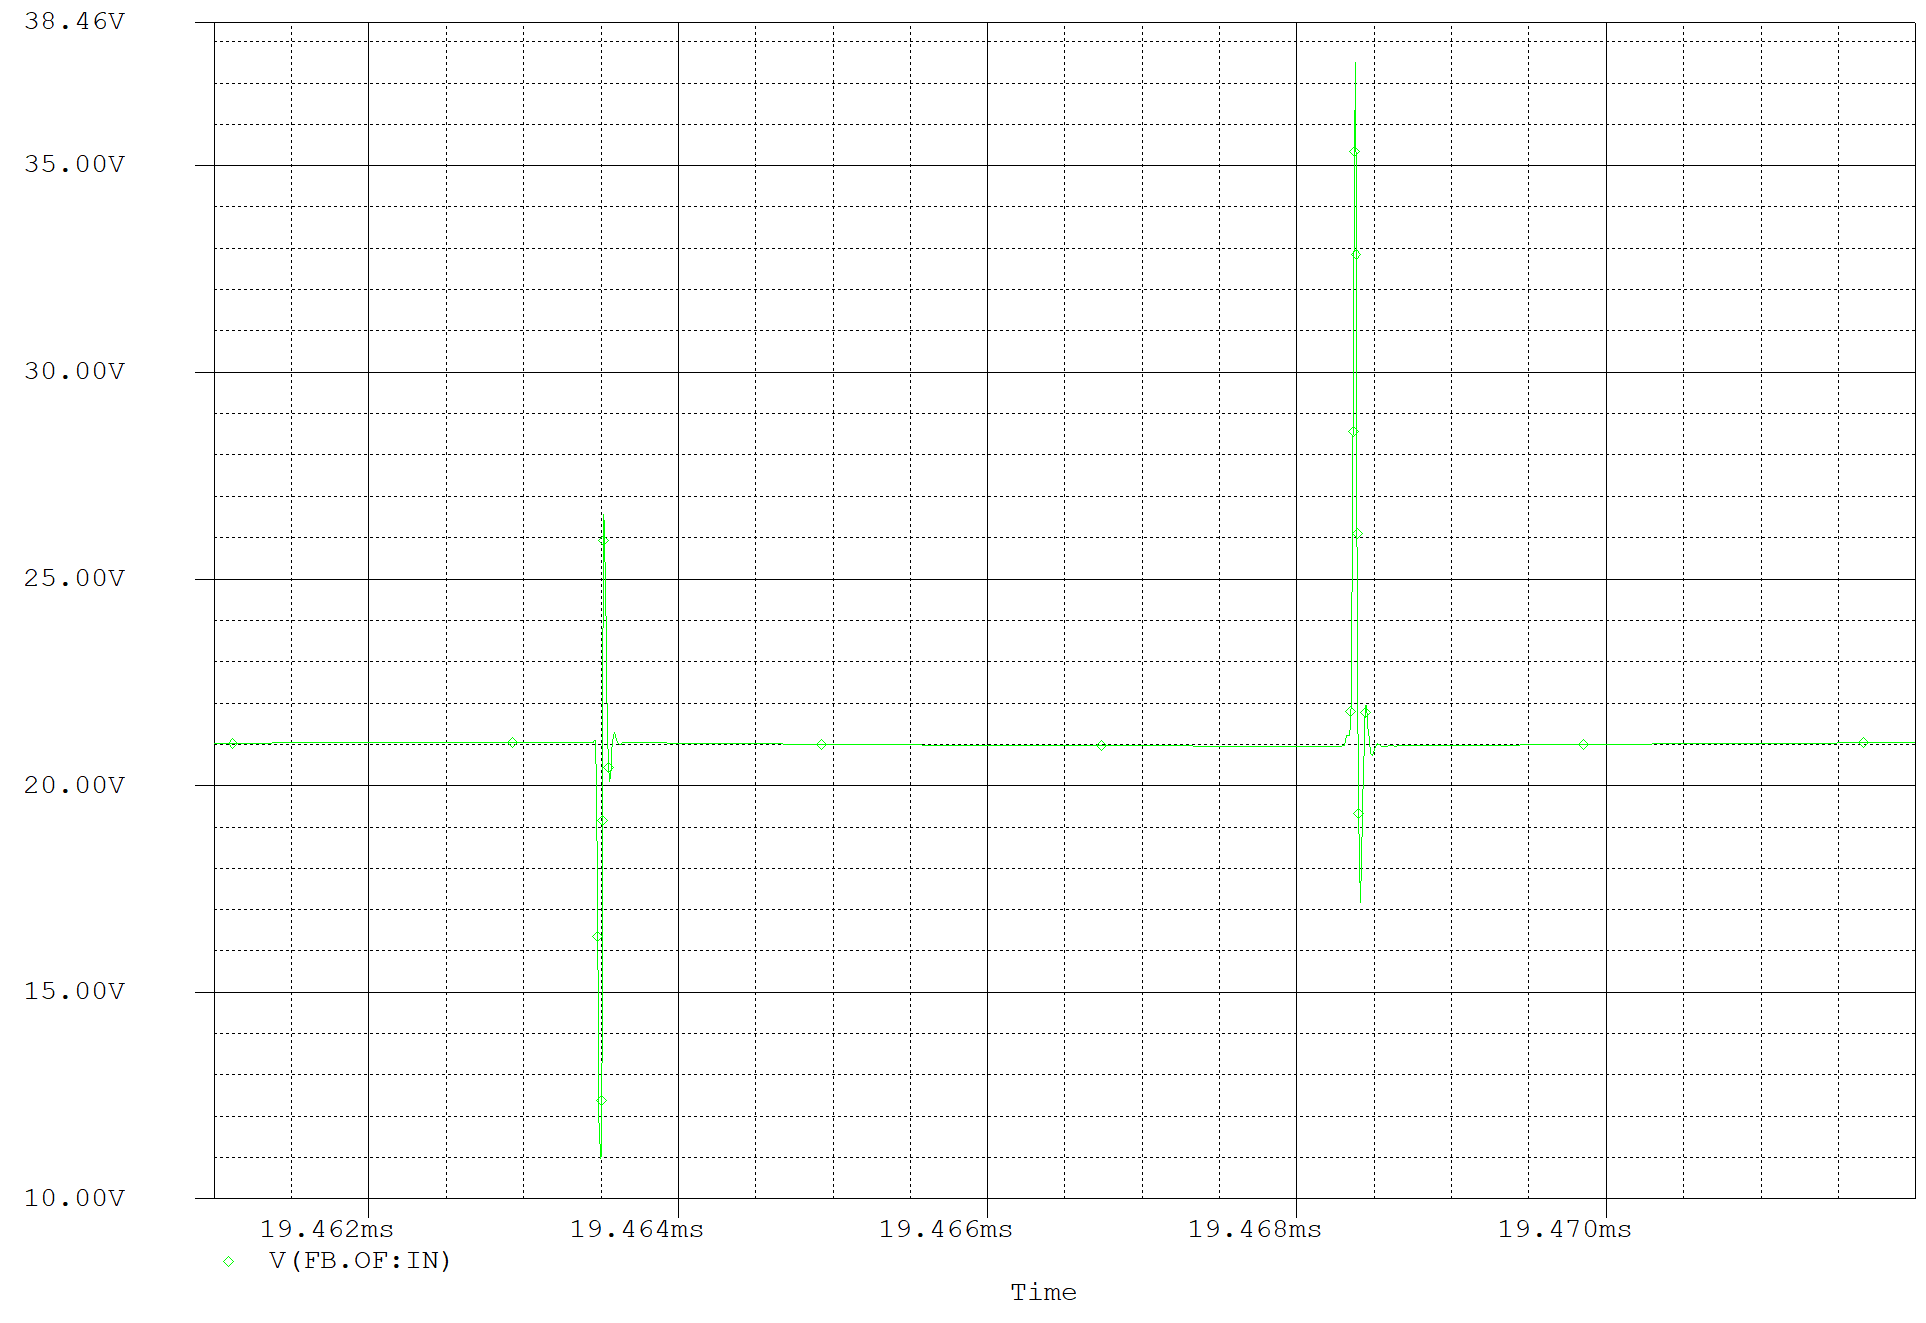
\includegraphics[max width=0.9\linewidth]{/tex/3iteration/billeder/Simulering/Simulering_udgangsfilter_U.png}
	\caption{Udgangssignal før filteret}
	\label{fig:simulering_udgangsfilter_U}
\end{figure}

\begin{figure}[H]
	\center
	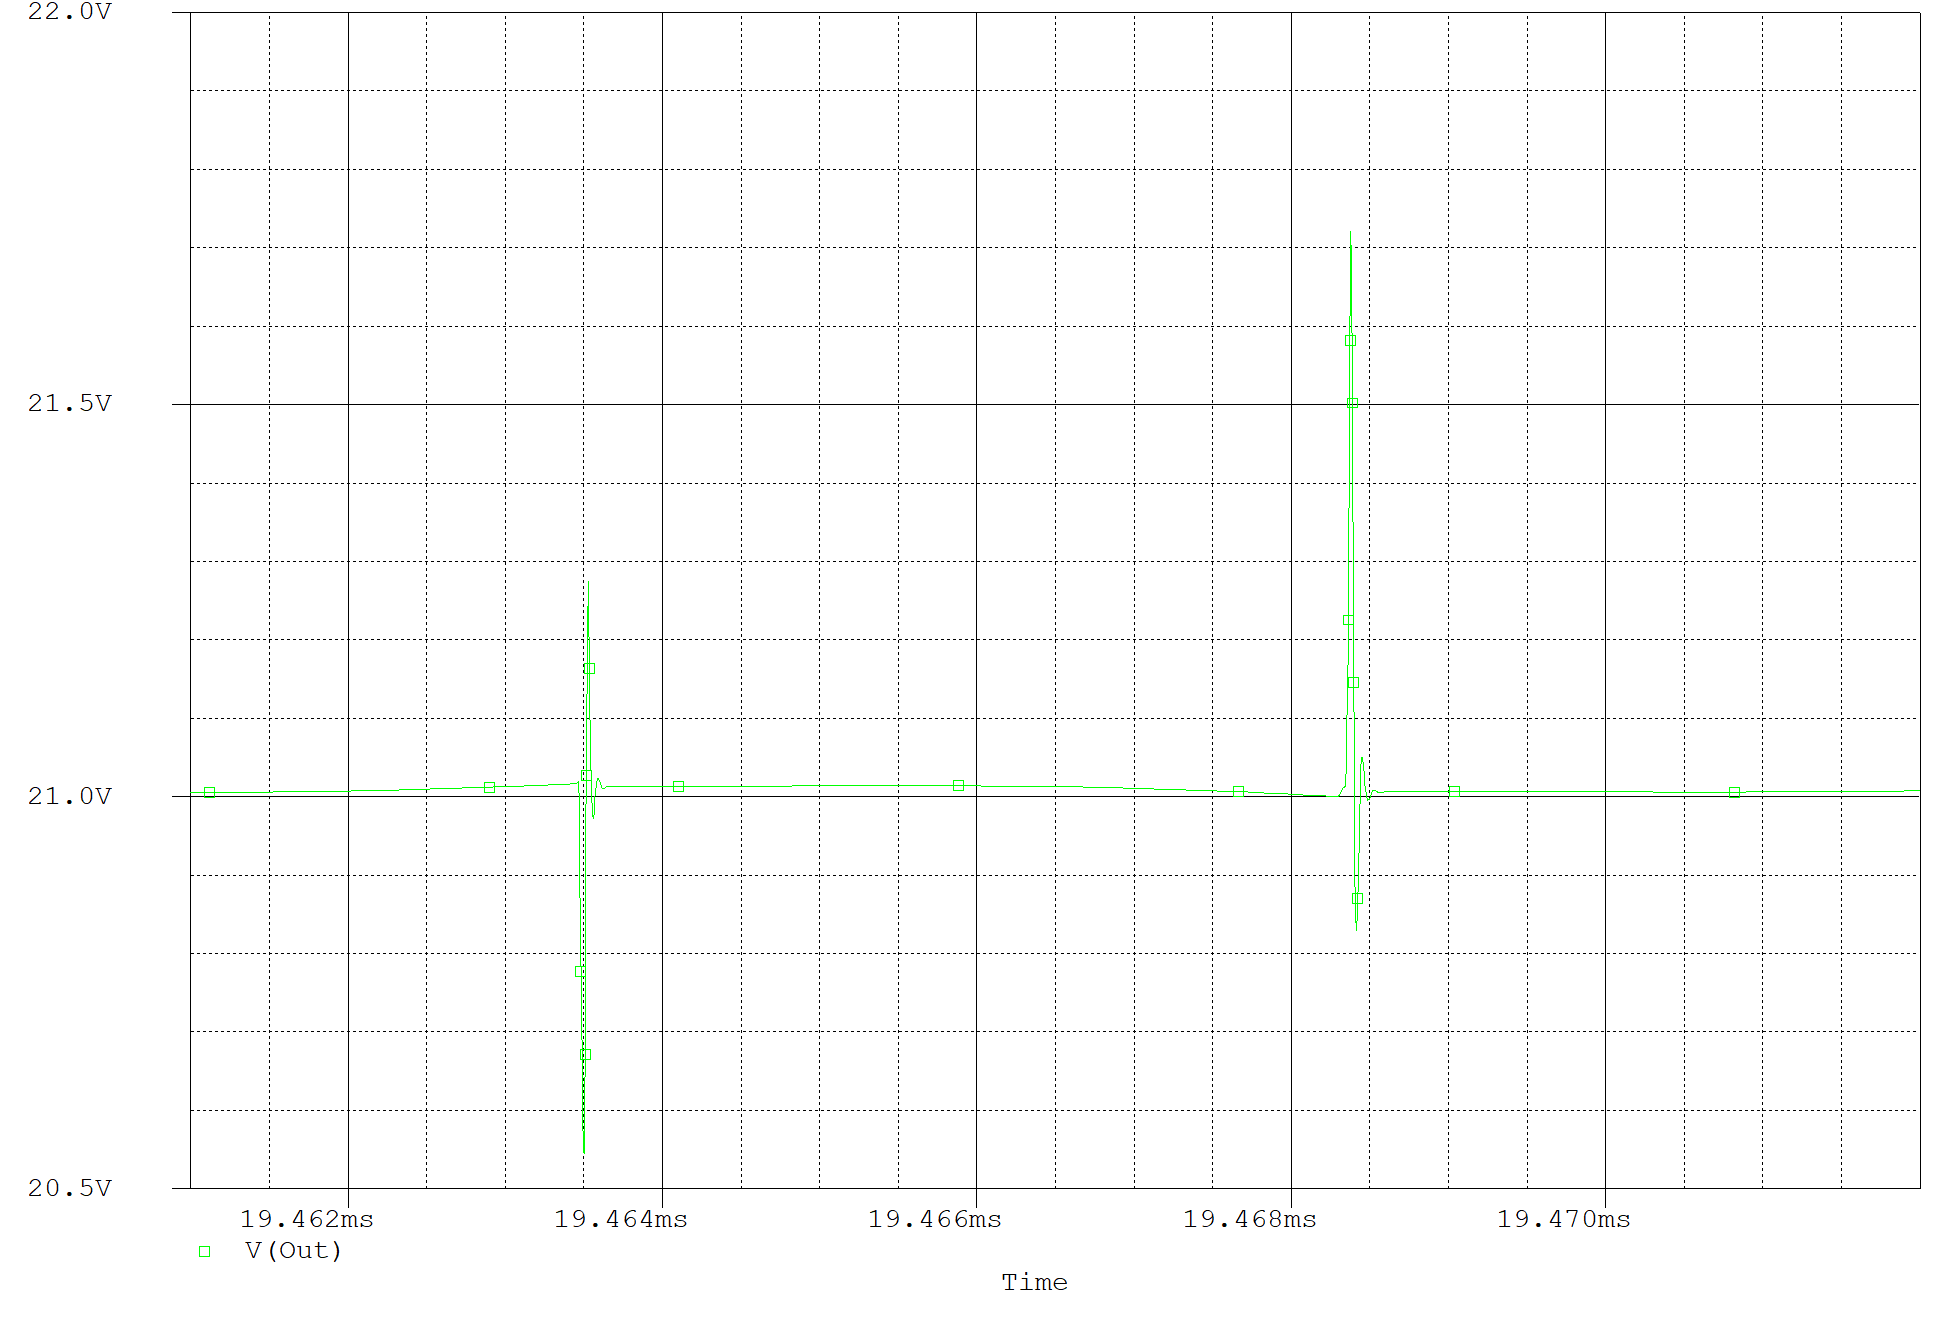
\includegraphics[max width=0.9\linewidth]{/tex/3iteration/billeder/Simulering/Simulering_udgangsfilter_M.png}
	\caption{Udgangssignal efter filteret}
	\label{fig:simulering_udgangsfilter_M}
\end{figure}
